\section{Measurements and data}
\label{sec:data}

\begin{figure}[pos=tbp]
\centering
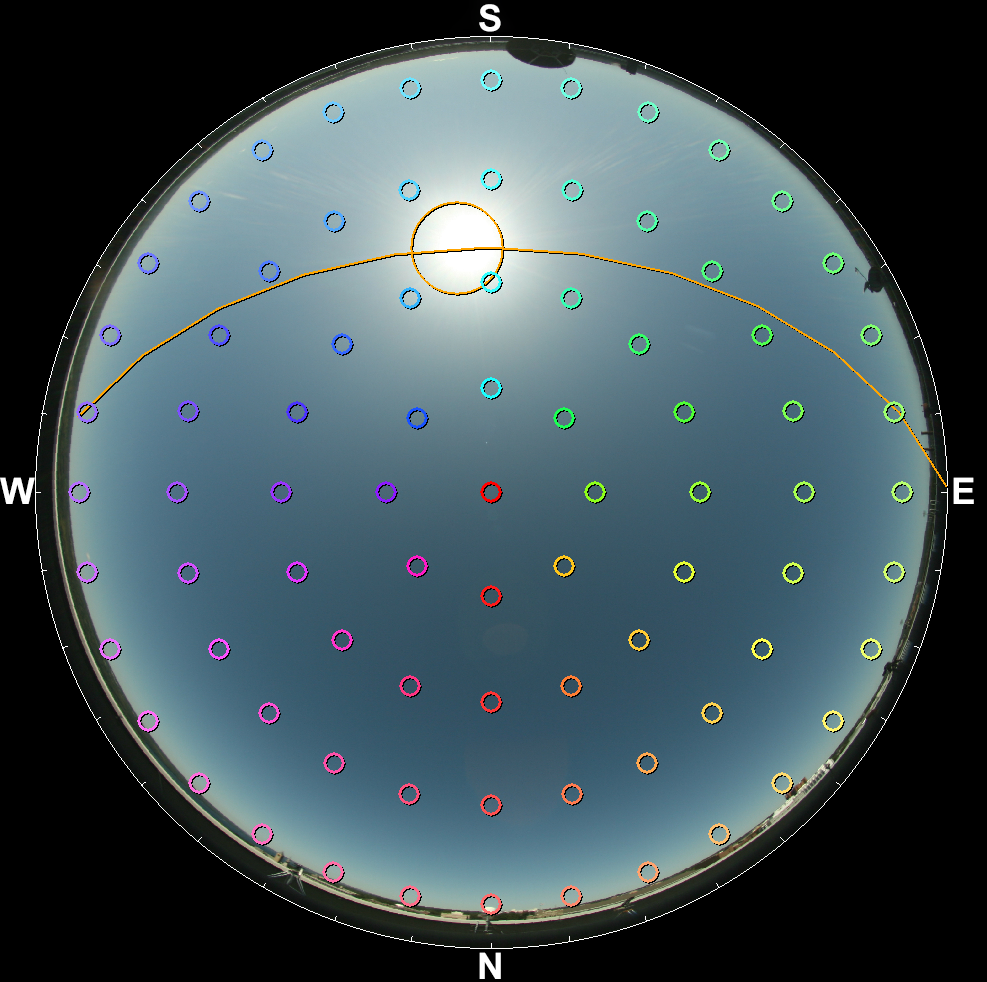
\includegraphics[width=0.325\textwidth]{img/capturesky.png}~%
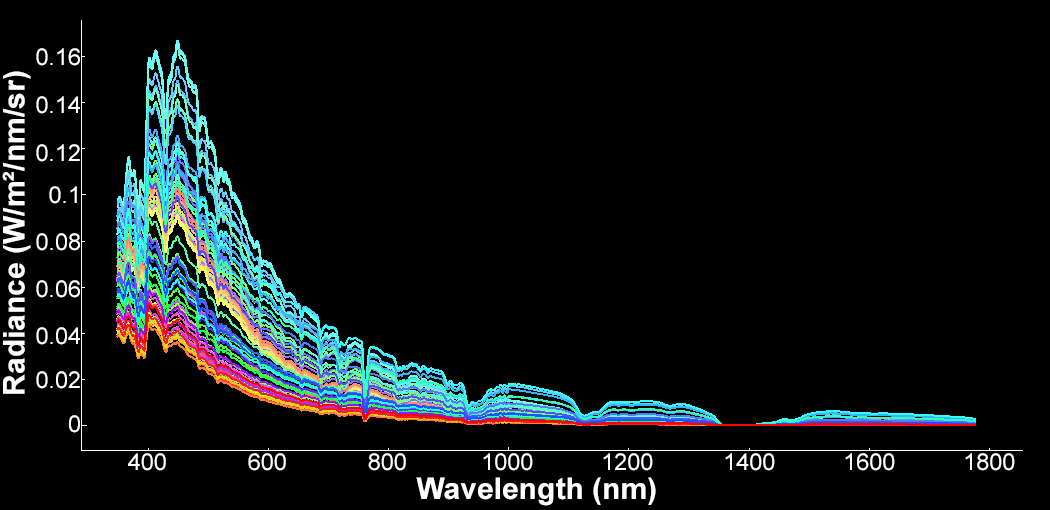
\includegraphics[width=0.665\textwidth]{img/capturerads.png}%,height=2.26in
\caption[A sky capture consists of HDR imagery and 81 radiance measurements]{A single sky capture consisted of high-resolution imagery and 81 spectral radiance measurements between 350-2500 nm (350-1780 nm used for this work). (a) shows the sky coordinate locations of the 81 radiance measurements projected onto a sky image; in other words, where in the sky each measurement was made. The sun's location and path is depicted in orange. (b) shows the correlating radiance measurement values in W~/~m\textsuperscript{2}~/~nm~/~sr between 350-1780 nm. The colors of each sky location in (a) correlate with radiance distributions in (b). As expected, radiance measurements taken closer to the sun are higher. The radius of colored circles is not to exact scale with sampled pixel area used in methods described in this work.}
\label{fig:skycapture}
\end{figure}

Measurements in this work come from the sky scanner discussed in detail by \citet{kider_framework_2014}. This framework captured high-resolution HDR imagery of the sky (8 exposures), along with atmospheric spectral radiance distributions (350-2500 nm) from 81 sample points in concentric circle patterns across the sky. Measurements were taken from the ground. The sampling pattern is arbitrary, but was designed to capture a uniformly distributed ``skeleton'' of measurements across the sky. The spectral radiance distributions were measured in W~/~m\textsuperscript{2}~/~nm~/~sr with an ASD FieldSpec Pro spectroradiometer through a 1\degree~solid angle fore-optic \citep{malthus_foreoptic}, and were validated against NASA datasets \citep{kider_framework_2014}. The multiple exposure photographs of the sky were captured in both CR2 (raw) and JPG formats consecutively at 4368~x~2912 pixels with a commodity Canon 5D digital single-lens reflex (DSLR) full-frame camera with underlying complementary metal-oxide-semiconductor (CMOS) image sensor, together with a Sigma 8 mm f/3.5 EX DG circular fisheye lens, and a Kodak Wratten neutral density filter. JPG compression quality level was set to 100. We automated the process with libgphoto2, which took approximately 40 s to capture all exposures and formats of photographs of the sky. Irradiance was also measured, but ignored for the purposes of this work.

All measurements were taken at a single site location, (42.44344, -76.48163) decimal degrees, on the rooftop of Frank Rhodes Hall, Cornell University, Ithaca, New York, USA. 453 total sky captures were taken over 16 days between 2012-2013, covering all four seasons, dawn to dusk, and various sky covers, for a total of over 36000 individual spectral radiance measurements. Roughly 25\% of the captures consisted of full clear skies (0 octas of clouds), from which 6006 individual clear sky samples were used for this work. Scattered and overcast skies were purposely left out of this work to focus our efforts. A complete table listing of all usable data that we captured can be found in \citet{delrocco_spie}. This dataset is freely available to the public through our project website.

Hemispherical sky coordinates are specified in (azimuth,~altitude) coordinates, where azimuth is an angle Eastward from North, and altitude is ($90\degree -$ zenith). Sky imagery is vertically flipped due to capture orientation. The correlation of validated radiance measurements and sky color at the same sky coordinates is explained in \autoref{ssec:lens} and \autoref{ssec:skycolor}.

\subsection{Sky cover}
\label{ssec:skycover}

\begin{figure}[pos=tbp]
\begin{center}
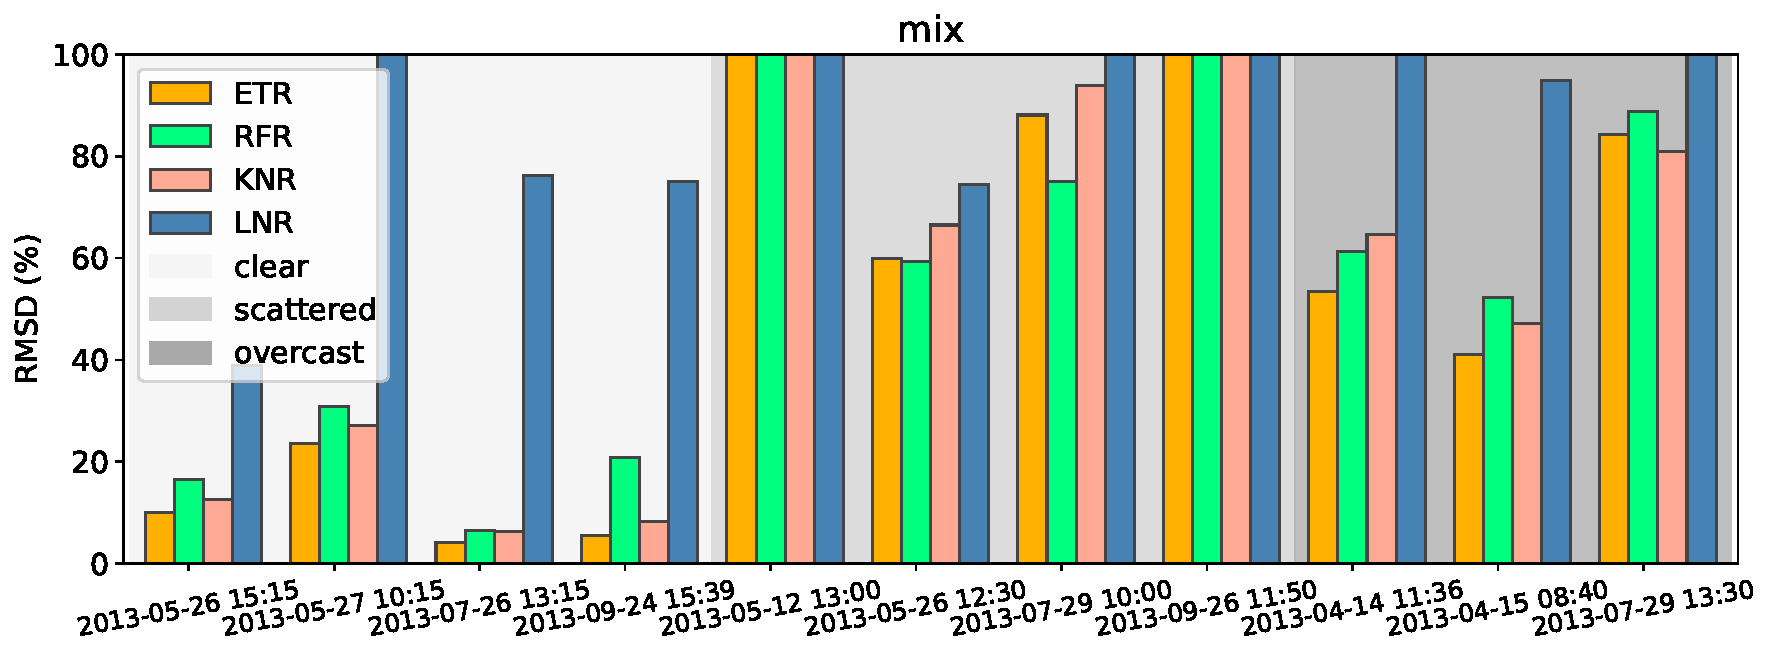
\includegraphics[width=0.98\textwidth]{img/results_prelim_mix.pdf}%
%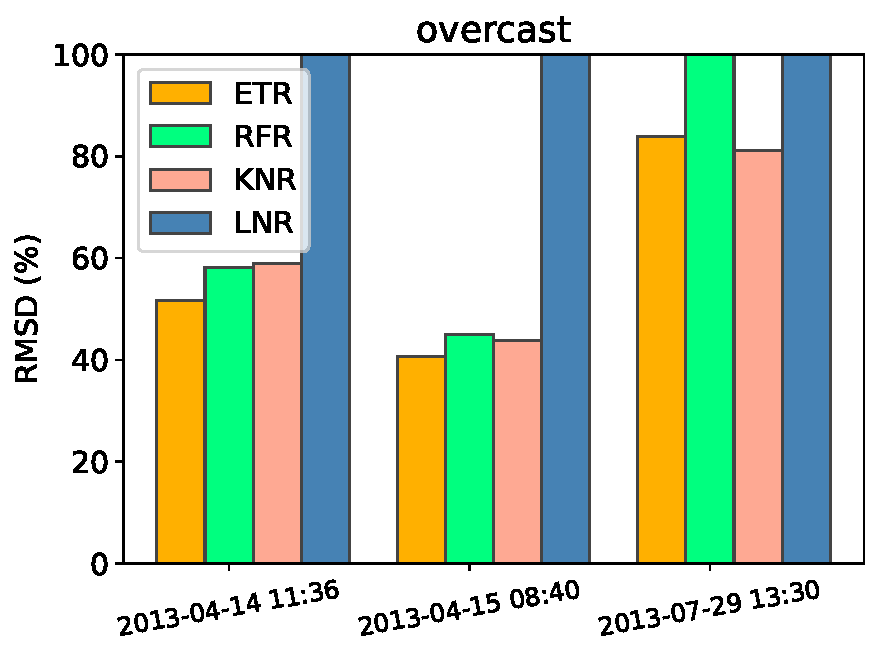
\includegraphics[width=0.4\textwidth]{img/results_prelim_overcast.pdf}%
\end{center}
\vspace{-2mm}
\caption[skycover]{Preliminary model results from \cite{delrocco_spie}, showing initial models trained and tested on our entire dataset of sky captures. The regression approach showed more promise on clear skies than scattered or overcast skies.}
\label{fig:skycover}
\end{figure}

As mentioned, our entire dataset includes a variety of sky cover conditions, roughly 25\% clear skies, 67\% scattered, and 8\% completely overcast. We assessed sky cover manually with our dataset browsing tool, even though procedural assessment is possible. We used the categorization of sky conditions provided by the US National Oceanic and Atmospheric Administration (NOAA) \citep{noaa_fmh1chpt9_2017}, designating skies as clear (CLR), scattered (SCT), and overcast (OVC). CLR and OVC skies contained 0 and 8 oktas of cloud cover, respectively. We used SCT for any sky with cloud coverage between 1-7 oktas. The distinction of few (FEW) and broken (BKN) skies was ignored to minimize the number of machine learning models necessary for downstream applications.

As discussed in our preliminary work \citep{delrocco_spie}, we initially trained and tested sky samples of all sky covers. We then found that our regression models performed dramatically better when tested on sky cover specific datasets. Although the models trained and tested on scattered and overcast skies could have been improved upon, we surmised for the time being that perhaps more modern techniques (e.g. deep learning neural networks) were best suited to model the likely non-linear relationships of scattered and overcast skies and spectral radiation. The work proposed here is our most refined approach of using regression models on clear skies specifically. This includes validation of our predictions with a validated radiative transfer software package, more experiments, spectral radiance predictions for every single pixel of a sky photo, the use of multiple exposures (HDR), the accommodation of lens linearity, sky samples within the circumsolar region, and more accurate whole sky error plots.

As the title of this work suggests, the regression model approach presented is currently not unified across all sky covers. The process of separating clear, scattered, and overcast skies has been discussed in many prior papers, using metrics such as clear-sky index, R/B ratio, fractional cloud cover, colormetric and spectral combined metric, etc. \citep{arking_cloudcover, lopez-alvarez_using_2008, cazorla_development_2008, yamashita_cloud, li_cloud, saito_cloud, nou_intrahour}. There are two valid procedural approaches to using our models. Either categorize the entire sky into buckets of CLR, FEW, BKN, SCT, OVC (or any other distinction), and use a capture of the sky with an appropriate model, or separate clear from cloudy samples from parts of each sky and pass samples to separate models for prediction.

\subsection{Lens linearity}
\label{ssec:lens}

\begin{figure}[pos=tbp]
\centering
\begin{overpic}[width=0.35\textwidth]{img/lenswarp.png}%
\put(20,850){(a)}%
\end{overpic}%
\hspace{0.3in}%
%\frame{
\begin{overpic}[width=0.35\textwidth]{img/lenswarp_plot.pdf}%
\put(-100,850){(b)}%
\end{overpic}%
%}
%\vspace{1mm}
\caption[The lens warp of our camera visualized]{This figure visualizes the linearity of our lens, or the differences (``lens warp'') between an ideal fisheye lens and the lens we used in this work. (a) plots the altitudes 12.1151\degree, 33.749\degree, 53.3665\degree, and 71.9187\degree~(altitudes of radiance measurements) for our actual lens (magenta) vs an ideal fisheye lens (white). The deviation, in terms of number of pixels, is not insignificant. The computed location and path of the sun, after lens correction, is overlaid (orange). (b) plots sample points from a lens linearity calibration experiment from our actual lens (solid line) vs an ideal fisheye lens (dashed line). The sample points of the solid line were used to fit \autoref{eq:lens_sigma}.}
\label{fig:lenswarp}
\end{figure}

Because our work involved mapping hemispherical sky coordinates to 2D pixel coordinates, and vice versa, it was important to accurately model the behavior of the fisheye lens employed. In a perfect circular fisheye lens, often called a "tru-theta" lens, equal increments in radius on the fisheye image correspond to equal angle increments of the respective field rays. Actual fisheye lenses typically exhibit some form of non-linearity, even those lenses designed to be linear \citep{bourke_fisheye}. Although more important with variegated skies (scattered, overcast, etc.), a measurement difference of even a single degree can result in sampling pixels in or out of the sun's corona. The standard ideal lens equation for mapping hemispherical sky coordinates to 2D center offset coordinates can be written as:
\begin{equation}
\label{eq:lens_ideal}
(x,~y) = \frac{2 \cdot zenith}{{\f}isheye{\f}ov} \cdot (\cos (azimuth) ,~\sin (azimuth))\textrm{.}
\end{equation}

The following procedure was used to measure the relationship between field angle and position on the image:
\begin{enumerate}[1.]
\item A close and distant vertical feature in the fisheye image was chosen. The zero parallax position of the lens is the position along the lens axis where those features stay aligned despite rotations perpendicular to the lens axis.
\item A clear narrow object in the image was chosen as a reference point and aligned with the center of fisheye image.
\item The lens is rotated in 5\degree~steps from 0 to 90\degree,~and a photograph taken.
\item For each photograph, the distance of the reference point from the center was measured.
\end{enumerate}
For our Sigma 8 mm f/3.5 fisheye lens, this resulted in the following non-linear curve (plotted in \autoref{fig:lenswarp}), which was then used to alter zenith of sky coordinates ($ r = zenith $):
\begin{equation}
\label{eq:lens_sigma}
r^{\prime} = 0.7230r + 0.0252r^2 - 0.0499r^3 - 0.0004325r^4\textrm{.}~
\end{equation}

\begin{figure}[pos=tbp]
% %\hspace{0.2mm}
% \begin{overpic}[width=0.325\textwidth]{img/sampling_angle.png}%
% \put(490,750){\small{Zenith}}
% \put(650,30){\small{North}}
% \put(560,170){\small{$P\theta$}}
% \put(590,295){\small{$P\phi$}}
% \put(760,175){\small{Pixels}}
% \put(180,280){\small{Fisheye}}
% \put(150,220){\small{sky image}}
% \put(625,540){\small{$L_{e\Omega\lambda}$}}
% %\put(650,500){\rotatebox{40}{\small{Radiance}}
% %------------
% \put(960,50){\linethickness{0.2mm}\color{white}\polygon*(0,0)(500,0)(500,500)(0,500)}%
% \put(960,50){\linethickness{0.2mm}\color{black}\polygon(0,0)(500,0)(500,500)(0,500)}%
% \put(960,150){\linethickness{0.2mm}\color{black}\line(1,0){500}}%
% \put(960,250){\linethickness{0.2mm}\color{black}\line(1,0){500}}%
% \put(960,350){\linethickness{0.2mm}\color{black}\line(1,0){500}}%
% \put(960,450){\linethickness{0.2mm}\color{black}\line(1,0){500}}%
% \put(1060,50){\linethickness{0.2mm}\color{black}\line(0,1){500}}%
% \put(1160,50){\linethickness{0.2mm}\color{black}\line(0,1){500}}%
% \put(1260,50){\linethickness{0.2mm}\color{black}\line(0,1){500}}%
% \put(1360,50){\linethickness{0.2mm}\color{black}\line(0,1){500}}%
% %------------
% \put(965,80){\scriptsize{.003}}%
% \put(965,180){\scriptsize{.013}}%
% \put(965,280){\scriptsize{.022}}%
% \put(965,380){\scriptsize{.013}}%
% \put(965,480){\scriptsize{.003}}%
% %------------
% \put(1065,80){\scriptsize{.003}}%
% \put(1065,180){\scriptsize{.059}}%
% \put(1065,280){\scriptsize{.097}}%
% \put(1065,380){\scriptsize{.059}}%
% \put(1065,480){\scriptsize{.003}}%
% %------------
% \put(1165,80){\scriptsize{.022}}%
% \put(1165,180){\scriptsize{.097}}%
% \put(1165,280){\scriptsize{.159}}%
% \put(1165,380){\scriptsize{.097}}%
% \put(1165,480){\scriptsize{.022}}%
% %------------
% \put(1265,80){\scriptsize{.003}}%
% \put(1265,180){\scriptsize{.059}}%
% \put(1265,280){\scriptsize{.097}}%
% \put(1265,380){\scriptsize{.059}}%
% \put(1265,480){\scriptsize{.003}}%
% %------------
% \put(1365,80){\scriptsize{.003}}%
% \put(1365,180){\scriptsize{.013}}%
% \put(1365,280){\scriptsize{.022}}%
% \put(1365,380){\scriptsize{.013}}%
% \put(1365,480){\scriptsize{.003}}%
% %------------
% \put(50,680){(a)}%
% \put(1360,590){(b)}%
% \end{overpic}\hfill
\begin{center}
\begin{overpic}[width=0.55\textwidth]{img/sampling.png}%
\put(30,480){(a)}%
\put(930,400){(b)}%
\end{overpic}
\end{center}
\vspace{-2mm}
\caption[skycolor]{Here we show the standard radiometry of measuring the steridian area of a single sky sample, one of 81 spectral radiance measurements at sky coordinate $(P\theta,P\phi)$ (azimuth, altitude), whose coordinate is then projected onto a 2D photo of the sky. (a) shows the captured steridian area projected onto the sky image, the bounds of which contain the pixels of interest for that sky sample; (b) shows the weights of a 5x5 Gaussian convolution matrix which is applied to the pixels in those bounds to compute a final color for that sky sample.}
\label{fig:skycolor}
\end{figure}

\subsection{Sky color sampling}
\label{ssec:skycolor}

Color at a particular location in the sky is a fairly subjective measure. What our eyes detect, what instruments measure, and how that data is processed, differs dramatically. Nevertheless, our research investigates the relationship between sky color and energy distribution, and thus a quantitative metric must be used.

To quantify sky color at specific points in the sky, we projected the bounds of a 1\degree~solid angle (same as fore-optic we used when measuring radiance) onto the 2D sky images captured with our digital camera (multiple images for the HDR experiment), and then sampled the pixel colors with a square convolution of similar width to the radius (\autoref{fig:skycolor}). In other words, when exporting data associated with a sky capture, we correlate the 81 radiance measurements with 81 pixel samplings of a sky photo, at the same lens linearity corrected coordinates projected to 2D.

More than a single pixel was used to estimate sky color at each sampled sky location because the corresponding spectral radiance measurement was captured within a 1\degree~steridian. To estimate the equivalent color, we used a common image processing technique known as convolution, which involves sliding a matrix of weights or homogeneous values (the kernel) over a set of image pixels in order to compute a new set of pixels \citep{parker_imgalgs}. Such convolutions are used to implement a wide variety of image filters like blurring, edge highlighting, etc. We used a Gaussian convolution, in particular, to blend the pixel colors together, weighting pixels closer to the center higher than pixels near the edges of the projected bounds.

We note that a square convolution does not account for all pixels in a projected circular area exactly; in fact, the projected circle becomes an increasingly oblong ellipse as altitude decreases. A rectangular convolution kernel would likely provide better coverage of the pixels in the projected bounds. Our kernel was chosen for real-time efficiency and overlap with existing image processing techniques and libraries, most of which use square kernels. The weights of our Gaussian kernels were generated with the following equation \citep{fisher_hipr}:
\begin{equation}
\label{eq:gaussian_kernel}
kernel(x,y) = \frac{1}{2 \pi \sigma^2} \cdot e^{-\frac{x^2 + y^2}{2 \sigma^2}}\textrm{,}~
\end{equation}

\noindent
with kernel dimensions relative to the bounds of the convolution, and a standard deviation ($\sigma$) of half the radius.

\subsection{Raw vs. digital positive}

\begin{figure}[pos=tbp]
\begin{center}
\begin{overpic}[width=0.3\textwidth]{img/positive_jpg.png}
\put(0,900){(a)}%
\end{overpic}%
~~~%
\begin{overpic}[width=0.3\textwidth]{img/positive_tiff.png}
\put(0,900){(b)}%
\end{overpic}%
\end{center}
\vspace{-2mm}
\caption[jpgvstiff]{{05/27/2013 09:00} 1s exposure of sky as a more traditional, camera processed, compressed JPG (a), and as a minimally processed, uncompressed TIFF (b). (a) approximates what humans see when looking at the sky, but (b) is more accurate in terms of what the DSLR CMOS sensor measures.}
\label{fig:jpg_vs_tiff}
\end{figure}

As mentioned, we captured photographs in a Canon CR2 (raw) format and a more traditional, camera processed, compressed JPG file format. Raw images contain much more capture information in a pre-interpolated format, before debayering, noise filtering, color space conversions, gamma correction, etc. In our previous work, we worked with the compressed JPG captures, which were smaller and faster to process \citep{delrocco_spie}. For this work, we strove for accuracy of recorded color values and interpolated the raw photographs into uncompressed TIFF files, using camera white balance, but no other post-processing options that digital cameras use to produce images closer to what humans see (e.g. gamma correction, additive brightness, exposure shift, etc.). We used rawpy to read and process the raw images \citep{riechert_rawpy, libraw}. \autoref{fig:jpg_vs_tiff} shows the difference. Our previous work already showed that it is possible to infer a relationship between sky appearance and spectral radiance using compressed imagery. The consistency of raw photograph interpolation may be more crucial than the specific parameters used.
